\section{微分}\label{zhang_differential}
%\begin{figure}[htp]
%    \centering
 %   \begin{tikzpicture}[>=latex]
      %\draw[-](0,0)--(3,0)--(3,3)--(0,3)--(0,0);
      %\draw[-](2,0)--(2,3);
    %  \draw[-](0,2)--(3,2);
   %   \node at(1,1){$A=x_0^2$};
  %\end{tikzpicture}
 % \end{figure}
  \subsection{定义}
  \begin{center}
    设函数$f(x)$在点$x_0$的一个邻域内有定义。$\vartriangle y=f(x_0+\vartriangle x)-f(x_0)$\\\
    如果$\vartriangle y$可以表示为$\vartriangle y=A\vartriangle x+\circ (\vartriangle x)$其中$A$为与$\vartriangle x$无关的常数\\
    则称$f(x)$在点$x_0$可微,$A\vartriangle x$称为$f(x)$在点$x_0$处的微分。\\
    $\mbox{记作:}dy=A\vartriangle x$
  \end{center}
\begin{figure}[htp]
   \centering
    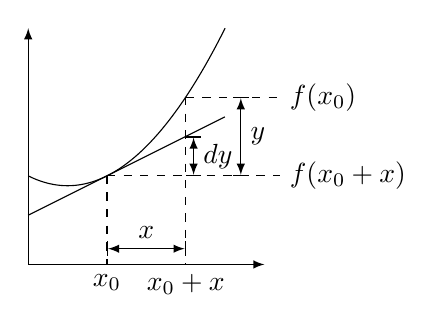
\begin{tikzpicture}[>=latex]
      \draw[->](0,0)--(3,0);
      \draw[->](0,0)--(0,3);
      \draw[domain=0:2.5,samples=1000] plot(\x,{((\x-.5)^2)*(1/2)+1});
      \draw[domain=0:2.5,samples=500] plot(\x,{(\x-1)*(1/2)+9/8});
      \draw[|<->|] (2.1,{(2-1)*(1/2)+9/8})--(2.1,{(((1-.5)^2)*(1/2)+1+(2-1)*(1/2)+9/8)/2})node[right]{$dy$}--(2.1,{((1-.5)^2)*(1/2)+1});
      \draw[dashed](1,{((1-.5)^2)*(1/2)+1})--(1,0)node[below]{$x_0$};
      \draw[dashed](2,{((2-.5)^2)*(1/2)+1})--(2,0)node[below]{$x_0+\vartriangle x$};
     % \node at (3,-1)[below]{常函数\ $f(x)=a\{a\in R\}$};
      \draw[|<->|] (1,.2)--(1.5,.2)node[above]{$\vartriangle x$}--(2,.2);
      \draw[dashed](2,{((2-.5)^2)*(1/2)+1})--(3.2,{((2-.5)^2)*(1/2)+1})node[right]{$f(x_0)$};
      \draw[dashed](1,{((1-.5)^2)*(1/2)+1})--(3.2,{((1-.5)^2)*(1/2)+1})node[right]{$f(x_0+\vartriangle x)$};
      \draw[|<->|](2.7,{((2-.5)^2)*(1/2)+1})--(2.7,{(((2-.5)^2)*(1/2)+1+((1-.5)^2)*(1/2)+1)/2})node[right]{$\vartriangle y$}--(2.7,{((1-.5)^2)*(1/2)+1});
    \end{tikzpicture}
\end{figure}
\begin{align}
    \mbox{可微}\Rightarrow\mbox{可导}\label{differential_to_derivative}\\
    \mbox{可导}\Rightarrow\mbox{可微}\label{derivative_to_differential}
\end{align}

\subsection{微分法则}
\subsubsection{核心根本}
\begin{figure}[htp]
    \centering
    \begin{tikzpicture}[>=latex]
      \draw[->](1.5,.2)--(1.5,.5)--(3,.5)--(3,.2);
      \node at(2.25,.5)[above]{积分};
      \draw[<-](1.5,-.2)--(1.5,-.5)--(3,-.5)--(3,-.2);
      \node at(2.25,-.5)[below]{求导};
      \node at(.5,0){$dy=$};
      \node at(1.5,0){$f'(x)$};
      \node at(2.3,0){$d$};
      \node at(3,0){$x$};
  \end{tikzpicture}
\end{figure}
\subsubsection{四则运算}
\begin{align}
    d\left(u\pm v\right)=du\pm dv\label{differential_operation_rule_1}\\
    d(uv)=vdu+udv \label{differential_operation_rule_2}\\
    d\left(\frac{u}{v}\right)=\frac{vdu+udv}{v^2} \label{differential_operation_rule_3}
\end{align}
\subsubsection{复合运算}
\begin{center}
    可微$\begin{cases}
        y=f(u)\\
        u=g(x)
    \end{cases}\Rightarrow \begin{cases}
        dy=f'(u)du\\
        du=g'(x)dx
    \end{cases}$则$y=f(g(x))$也可微\\
    且$  dy=f'(u)du=f'(u)g(x)dx$\\
    $u$是否为中间变量都成立,微分的不变性。
\end{center}
\subsubsection{近似计算公式}
\begin{center}
    $\vartriangle x\rightarrow 0, dy\approx \vartriangle y\begin{cases}
        dy=f'(x_0)\vartriangle x\\
        \vartriangle y=f(x_0+\vartriangle x)-f(x_0)
    \end{cases}\begin{cases}
        f(x_0+\vartriangle x)\approx f(x_0)+f'(x_0)\vartriangle x\\
        f(x)\approx f(x_0)+f'(x_0)(x-x_0)\\
        x_0=0\begin{cases}
            f(x)\approx f(0)+f'(0)x\\
            \sqrt{n}\approx 1+\frac{1}{n}x\\
            \sin x \approx x\\
            \tan x \approx x\\
            e^x \approx 1+x\\
            \ln(1+n)\approx x
        \end{cases}
    \end{cases}$\\
\end{center}
\subsubsection{奇偶函数导数}
\begin{center}
    偶函数导数为奇函数$f(x)=f(-x)\Leftrightarrow f'(x)=-f'(-x)$\\
    奇函数导数为偶函数$f(x)=-f(-x)\Leftrightarrow f'(x)=f'(-x)$
\end{center}
\subsubsection{区间恒为0}
$$\mbox{若}f'(x)\mbox{在区间恒为零,则}f(x)\mbox{在区间}I\mbox{上为一常数}$$
$\mbox{设}x_1,x_2\mbox{为区间}I\mbox{内任意两点}x_1<x_2$\\
$f(x_2)-f(x_1)=f'(\xi)(x_2-x_1)\equiv 0 $\\
$f(x_2)\equiv f(x_1)=C$
\subsection{中值定理}
\subsubsection{费马引理}
\begin{center}
    $f(x)\qquad \forall x\in \mathring{U}(x_0)\begin{cases}
        f(x)\leqslant f(x_0)\qquad f(x)\mbox{在}x_0\mbox{处取极大值}\\
        f(x)\geqslant f(x_0)\qquad f(x)\mbox{在}x_0\mbox{处取极小值}
    \end{cases}$
\end{center}
\begin{equation}
    \mbox{如果可导函数}y=f(x)\mbox{在}x_0\mbox{取极值,则}f'(x_0)=0\label{Fermat_Lemma}
\end{equation}
\subsubsection{罗尔定理}
\begin{center}
    $\mbox{如果函数}f(x)\mbox{满}\begin{cases}
    \mbox{在闭区间$\left[a,b\right]$上连续}\\
    \mbox{在开区间(a,b)可导}\\
    f(a)=f(b)
    \end{cases}$\\
    \begin{align}
        \mbox{则至少有一点}\xi\in(a,b),f'(\xi)=0\label{Rolle's theorem}
    \end{align}
\end{center}
\begin{figure}[htp]
    \centering
    \begin{tikzpicture}[>=latex]
        \draw[->](-.5,0)--(8,0)node[right]{$x$};
        \draw[->](0,-.5)--(0,4)node[above]{$y$};
        \draw[domain=0:2*pi,samples=1000] plot(\x+1,{sin(\x r)+2});      
        \draw[dashed] (1,{2})--(1,0)node[below]{$a$};    
        \draw[dashed] ({1+(2*pi)},{2})--({1+(2*pi)},0)node[below]{$b$};   
        \draw[dashed] (1,{2})node[left]{$A$}--({1+(2*pi)},{2})node[right]{$B$};
        \draw[dashed] ({1+(.5*pi)},{sin(pi/2 r)+2})--({1+(.5*pi)},0)node[below]{$\xi$};
        \draw[dashed] (1.5,{sin(pi/2 r)+2})--({.5+pi},{sin(pi/2 r)+2});
    \end{tikzpicture}
\end{figure}
\subsubsection{拉格朗日定理$\left(\mbox{微分中值定理}\right)$}
\begin{figure}[htp]
    \centering
    \begin{tikzpicture}[>=latex]
        \draw[->](-.5,0)--(8,0)node[right]{$x$};
        \draw[->](0,-.5)--(0,4)node[above]{$y$};
        \draw[domain=0:2*pi,samples=1000] plot(\x+1,{sin(\x r)+(\x/2)+1});
        \draw[dashed](1,1)--(1,0)node[below]{$a$};
        \draw[dashed]({1+(2*pi)},{(2*pi/2)+1})--({1+(2*pi)},0)node[below]{$b$};
        \draw[dashed](1,1)--({1+(2*pi)},{(2*pi/2)+1});
        \draw[dashed]({1+(pi/2)},{sin(pi/2 r)+(pi/4)+1})--({1+(pi/2)},0)node[below]{$\xi$};
        \draw[dashed]({1+(pi/2)-1},{sin(pi/2 r)+(pi/4)+1-.5})--({1+(pi/2)+1},{sin(pi/2 r)+(pi/4)+1+.5});
    \end{tikzpicture}
\end{figure}
\begin{center}
    $\mbox{如果函数}f(x)\mbox{满}\begin{cases}
    \mbox{在闭区间$\left[a,b\right]$上连续}\\
    \mbox{在开区间(a,b)可导}
    \end{cases}$\\
    $\mbox{则至少有一点}\xi\in(a,b)$\\
    \begin{align}
        f'(\xi)=\frac{f(b)-f(a)}{b-a}\Leftrightarrow f(b)-f(a)=f'(x)(b-a)\label{Lagrange's theorem}
    \end{align}
    在区间$\left[x,x+\vartriangle x\right]$用拉格朗日定理。\\
    $f(x+\vartriangle x)-f(x)=f'(\xi)\vartriangle x$\\
    $\xi\in(x,x+\vartriangle x)$记作:\ $\xi=x+\theta \vartriangle x\qquad 0<\theta <1$\\
    $f(x+\vartriangle x)-f(x)=f(x+\theta \vartriangle x)\vartriangle x$\\
    $\vartriangle y=f(x+\theta \vartriangle x)\vartriangle x$\\

\end{center}
\subsubsection{柯西定理}
